\chapter{Connectedness}\label{chp:2_4}


Connectedness is one of the simplest/most useful topological properties. It is intuitive and is relatively easy to understand, and, it is a powerful tool in proving many
well-known results, e.g. the intermediate value theorem.

For topological spaces which have simple pictures, it is easy to tell whether the space
is connected or not. But for more complicated spaces, it may be more complicated to
tell whether the space is connected or not.

\begin{figure}[htbp]
    \centering
    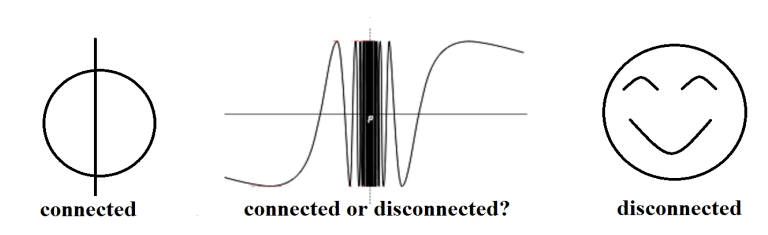
\includegraphics[width=0.6\textwidth]{figure/connectedness.png}
    \caption{}
\end{figure}

So we need a rigorous definition of connectedness (via the collection of open sets).
Before we give such a rigorous definition, let’s first look at a couple sets in $\R$
\begin{align*}
    (a)\  (0,3)\ (b)\ (0,1)\cup [2,3)\ (c)\ (0,1)\cup (1,3]\ (d)\ (0,1]\cup (1,3)
\end{align*}
Of course $(a)$ is connected, 
$(b)$ and $(c)$ are disconnected, 
while $(d)$ is connected! 
Although $(d)$ looks like a union of two intervals, they are really one interval $(0, 3)$ written
as a disjoint union of two subsets. The two subsets (0, 1] and (1, 3) are “attached”
together at the point 1, which is an element of (0, 1], but sits inside the closure of
(1, 3]. For the case (c), although the two “components” (0, 1) and (1, 3] sit “next to
each other”, it is still disconnected because (0, 1) contains no element in the closure of
(1, 3], and (1, 3] contains no element in the closure of (0, 1).
This example motivates us to define connectedness. Unlike most other conceptions
that you learned, connectedness is defined by its opposite. 

\section{Connectedness: The definition}
\begin{definition}{}{}
    Let $(X,\tau)$ be  topological space.\\
    (1) We say $X$ is disconnected, if there exists non-empty sets $A,B\subset X$ such that 
    \begin{align*}
        X=A\cup B \text{ and } A\cap \overline{B}=\overline{A}\cap B=\O.
    \end{align*}    
    (2) We say $X$ is connected if it is not disconnected.\\
    (3) We say a subset $X$ is connected/disconnected if it is connected/disconnected with respect to the subspace topology.
\end{definition}
\begin{remark}
    Note that by definition, the empty set is connected!
\end{remark}
\begin{remark}
    Suppose $A\subset X$ be a subset, then we say $A$ is connected if, 
    when endowed with the subspace topology, $(A,\tau_A)$ is connected. 
\end{remark}

\begin{proposition}{}{}
    Let $X$ be a topological space.
    Let $A\subset B\subset X$.
    Then $A$ is connected in B iff $A$ is connected in $X$.
\end{proposition}

\begin{proof}
    Let $\tau_A$ be the subspace topology on $A$ induced by $\tau$.
    Let $\tau_A'$be the subspace topology on $A$ induced by $\tau_B$.
    Then $A$ is connected in $X$ iff $(A,\tau_A)$ is connected.
    Similarly, $A$ is connected in $B$ iff $(A,\tau_A')$ is connected.
    By proposition\ref{prop:Subspace of Subspace is Subspace}, $\tau_A=\tau_A'$.
    Hence, $A$ is connected in $X$ iff $A$ is connected in $B$.
\end{proof}

\section{Connectedness: Equivalent characterizations.}

The definition above is intuitive but is also a little bit complicated. Fortunately
we have several other equivalent ways to describe connectedness.


\begin{proposition}{}{}
    For a topological space $X$, the following are equivalent:\\
    (1) $X$ is disconnected;\\
    (2) there exists non-empty disjoint open sets $A,B\subset X$ s.t. $X=A\cup B$;\\
    (3) there exists non-empty disjoint closed sets $A,B\subset X$ s.t. $X=A\cup B$;\\
    (4) there exists $A\neq \O$, $A\neq X$ such that $A$ is both open and closed in $X$.
\end{proposition}

\begin{proof}
    $(2)\Leftrightarrow (3)\Leftrightarrow (4)$ because
    \begin{align}
        A\cap B=\O \Leftrightarrow A^c=B, B^c=A.
    \end{align}
\end{proof}

\begin{proposition}{}{}
    For a topological space $X$, the following are equivalent:\\
    (1) $X$ is connected;\\
    (2) there is no non-empty disjoint open sets $A,B\subset X$ s.t. $X=A\cup B$;\\
    (3) $X$ and $\O$ are the only sets which are both open and closed in $X$.
\end{proposition}


\section{Examples of connected and disconnected spaces}
\begin{example}{}{}
    $(X,\tau_t)$ is connected, while $(X,\tau_s)$ is disconnected for $|X|\geqs 2$.
\end{example}

\begin{example}{}{}
    Infinite set with cofinite topology is connected.
\end{example}
\begin{proof}
    Let $(X,\tau_f)$ be an infinite set with cofinite topology. 
    Suppose $(X,\tau_f)$ is disconnected, then 
    $\exists$ non-empty open sets $A,B\subset X$ s.t. $A\cap B=\O$ and $X=A\cup B$.
    Then $X=\O^c=(A\cap B)^c=A^c\cup B^c$. Since $A,B$ is open in $(X,\tau_f)$, it follows that $A^c,B^c$ is finite and so $X$ is finite, 
    contradicting with the fact $X$ is infinite.
\end{proof}

\begin{example}
    Let $(X,\tau_c)$ be a co-countable topological space. 
    Show that $X$ is connected iff it is uncountable.
\end{example}
\begin{proof}
    ($\Leftarrow$):
    Suppose $(X,\tau_c)$ is disconnected when $X$ is uncountable, then 
    $\exists$ non-empty open sets $A,B\subset X$ s.t. $A\cap B=\O$ and $X=A\cup B$.
    Then $X=\O^c=(A\cap B)^c=A^c\cup B^c$. Since $A,B$ is open in $(X,\tau_c)$, 
    it follows that $A^c,B^c$ is countable and so $X$ is countable, 
    contradicting with the fact $X$ is uncountable.
\end{proof}


\begin{example}{}{}
    $\Q\subset \R$ is disconnected.
\end{example}

$\Q=((-\infty, -\sqrt{2})\cap \Q)\cup ((-\sqrt{2},+\infty)\cap \Q)$.

\begin{example}{}{}
    $S^1$(the unit circle in $\R^2$) is connected.
\end{example}

\begin{example}{}{}
    More generally, if $A \subset \R^2$ is countable, then $R^2 \setminus A$ is connected. 
    In particular, $R^2 \setminus Q^2$ is connected. 
    (Careful, this is not the set of all points with both coordinates irrational; it is
    the set of points such that at least one coordinate is irrational.)
\end{example}

\section{Connectedness in $\R$}

\begin{definition}{}{}
    A subset $S$ of $\R$ is said to be an interval if it has the following property: 
    if $x,z\in S$ and $y\in \R$ are such that $x<y<z$, then $y\in S$.
\end{definition}
\begin{remark}
    Each singleton set $\{x\}$ is an interval.
\end{remark}

\begin{remark}
    Every interval has one of the following forms: 
    $\{a\}$, $[a,b]$, $(a,b)$, $[a,b)$, $(a,b]$, $(-\infty,a)$, $(-\infty,a]$, $(a,\infty)$, $[a,\infty]$, $(-\infty,\infty)$.
\end{remark}

\begin{proposition}{}{}
    $\R$ is connected with respect to the euclidean topology.
\end{proposition}

\begin{proof}
    Suppose $\R$ is disconnected. Then there exists an open set 
\end{proof}

\begin{remark}
    By the same proof, one can show that all intervals
$(a, b)$, $[a, b]$, $(a, b]$, $[a, b)$,$(a,+\infty)$, $[a, +\infty)$,$(-\infty, b]$,
$(-\infty, b)$,$(-\infty, +\infty)$.
are connected.
\end{remark}









\section{Properties of connected spaces}
\subsection{Generalized intermediate value theorem}
\begin{proposition}{}{}
    Suppose $f:X\rightarrow Y$ is continuous. 
    Then for any connected subset $A\subset X$, 
    the image $f(A)\subset Y$ is connected.
\end{proposition}

\begin{proposition}{}{}
    A subspace of $R$ is connected if and only if it is an interval.
\end{proposition}

\begin{corollary}
    If $f:X\rightarrow Y$ is a homeomorphisom, then $X$ is connected iff $Y$ is connected.
\end{corollary}

\begin{corollary}{}{}
    If $X$ is connected, $f:X\rightarrow \R$ is continous, 
    and if there exist $x_1,x_2\in X$ s.t. $f(x_1)=a<b=f(x_2)$,
    then for any $a<c<b$, there exists $x\in X$ s.t. $f(x)=c$.
\end{corollary}

\subsection{The closure}

\begin{lemma}{}{connected subset with clopen subset}
    Let $X_0\subset X$ be both open and closed and $A\subset X$ be connected. 
    Then either $A\cap X_0=\O$ or $A\subset X_0$.
\end{lemma}

\begin{proof}
    If $X_0$ is both open and closed in $X$, then $A\cap X_0$ is both open and closed in $A$.
    Since $A$ is connected, it follows that the only sets which is both open and closed in $A$ is $A$ and $\O$.
    Then either $A\cap X_0=\O$ or $A\cap X_0=A$(implies $A\subset X_0$).
\end{proof}

\begin{proposition}{}{}
    If $X$ has a connected dense subset, then $X$ is connected.
\end{proposition}
\begin{proof}
    Suppose $A$ is a connected dense subset of $X$ and $X_0$ is a subset which is both open and closed.
    If $X_0\neq \O$, then $X_0\cap A\neq \O$, by lemma\ref{lem:connected subset with clopen subset}, $A\subset X_0$. 
    Then $X=\overline{A}\subset \overline{X_0}=X_0$. Then the only sets which is both open and closed in $X$ are $X$ and $\O$.
    Hence, $X$ is connected.
\end{proof}

\begin{corollary}{}{}
    Let $A$ be a connected subset of $X$. If $A\subset Y\subset \overline{A}$, then $Y$ is connected.
\end{corollary}
\begin{proof}
    Since $\text{cl}_Y(A)=Y\cap \text{cl}_X(A)=Y$, it follows that $A$ is a connected dense subset of $Y$ and so $Y$ is connected. 
\end{proof}

\begin{corollary}{}{}
    If $A$ is connected, so is $\overline{A}$.
\end{corollary}
\begin{proof}
    $A\subset \overline{A}\subset\overline{A}$.
\end{proof}

\begin{corollary}{Topologist's sine curve}{Topologist's sine curve is connected}
    The set 
    \begin{align*}
        S=\{(x,y):x\in (0,1),y=sin\frac{1}{x}\}\cup \{(0,y):y\in [-1,1]\}\subset \R^2
    \end{align*}
    is connected.
\end{corollary}

\subsection{The union}

\begin{proposition}{}{}
    Let $A_{\alpha}\subset X$ be a collection of non-empty connected subsets in $X$, 
    and assume $\cap_{\alpha}A_{\alpha}\neq \O$. Then $\cup_{\alpha}A_{\alpha}$ is connected. 
\end{proposition}
\begin{proof}
    Denote $Y=\cup_{\alpha}A_{\alpha}$. 
    Suppose $X_0$ is both open and closed in $Y$, we should show that $X_0=\O$ or $Y$.
    
\end{proof}

\section{The product}
\begin{proposition}{}{}
    If $X$, $Y$ are connected, so is $X \times Y$ .
\end{proposition}


\section{Locally connected}

\begin{definition}{}{}
    A topological space $X$ is locally connected at a point $x\in X$ if every neighbourhood $U$ of $x$ contains a connected neighbourhood $K$ of $x$.
    The space $X$ is locally connected if it is locally connected at every point $x\in X$.
\end{definition}


\section{Exercise}

\begin{exercise}{}{}
    Open subset of locally connected space is locally connected.
\end{exercise}

% \begin{proof}
%     Suppose $X$ is locally connected and $A\subset X$ is open. 
%     To show that $(A,\tau_A)$ is a locally connected topological space, 
%     we must prove that every neighbourhood $U$ of $x\in A$ contains connected elements of $\tau_A$, which implies $U$ contains a connected neighbourhood of $x$.
%     Since $X$ is locally connected, there exists $\tilde{\mathcal{B}}=\{O_{\alpha}\in \tau:\alpha\in I\}$ 
%     in which $O_{\alpha}$ is connected and $O_{\alpha}$ contains $x$ such that $x\in O_{\alpha}\subset U$ for some $\alpha\in I$.
%     Let $\mathcal{B}=\{O_{\alpha}\cap A:\alpha\in I\}$. We claim that $\mathcal{B}$ is a neighbourhood basis of $x$ in $A$.
%     In fact, Let $N\in \tau_A$ such that $x\in N$, then $\exists K\in \tau$ such that $N=K\cap A$. Then $N\in \tau$ as $K,A\in \tau$.
%     Then one can find $\alpha\in I$ such that $x\in O_{\alpha}\subset N$. Then $O_{\alpha}\cap A\subset N\cap A$. 
%     Since $N\subset A$, it follows that $O_{\alpha}\cap A\subset N$ as required. 
%     Now we use $\mathcal{B}$ to construct a connected neighbourhood basis of $x$.
%     Define $\phi:\mathcal{B}\rightarrow I$ such that $O_{\phi(N)}\subset N$. 
%     $O_{\phi(N)}\in \tau$ and $O_{\phi(N)}\subset N\subset A$. Then $O_{\phi(N)}=O_{\phi(N)}\cap A\in \tau_A$.
%     Since $O_{\phi(N)}$ is connected in $X$ and $O_{\phi(N)}\subset A$. Then $O_{\phi(N)}$ is connected in $A$.
%     Then for any $V\in\tau_A$ such that $x\in V$, there exist $N\in \mathcal{B}$ such that $x\in O_{\phi(N)}\subset N\subset V$
% \end{proof}

\begin{proof}
    Suppose $(X,\tau)$ is locally connected and $A\subset X$ is open. 
    For $x\in A$ and any neighbourhood $N$ of $x$ in $A$, $\exists U\in \tau_A$ such that $x\in U\subset N\subset A$.
    Then $U=O\cap A$ where $O\in \tau$. Then $U\in \tau$. Then $N$ is neighbourhood of $x$ in $X$.
    Since $X$ is locally connected, it follows that there exists connected neighbourhood $K$ of $x$ in $X$ and $V\in\tau$ such that 
    $x\in V\subset K\subset N\subset A\subset X$. 
    Then $K$ is connected in $A$ and $V=V\cap A\in\tau_A$. 
    Hence, K is a connected neighbourhood of $x$ in $A$.
    and so $A$ is locally connected.
\end{proof}

\begin{exercise}{P66 T7}{}
    $X$ is disconnected $\Leftrightarrow$ there exists a continuous function $f:X\rightarrow E^1$
    such that $f(X)$ only has two points.
\end{exercise}

\begin{proof}
    ($\Rightarrow$): If $X$ is disconnected, then there exists non-empty open sets $U,V$ s.t. 
    $X=U\cup V$ and $U\cap V=\O$. Define $f:X\rightarrow E^1$ such that $f(U)=0$ and $f(V)=1$.
    We claim that $f$ is continuous. For any open set $W$ in $E^1$, 
    if $0,1$ are not in $W$, then $f^{-1}(W)=\O$, which is open. If $0\in W$, $f^{-1}(W)=U$ which is open. 
    If $1\in W$, then $f^{-1}(W)=V$ which is open. Hence, $f$ is continous.
    \\
    ($\Leftarrow$): Suppose $X$ is connected. Since $f$ is continous, it follows that $f(X)$ is connected.
    But $f(X)=\{a,b\}$ ($a,b\in E^1$) is disconnected. 
\end{proof}

\begin{exercise}{P66 T8}{}
    Let $X$ be a subset of $E^2$ and $X=\{(x,y): \text{ not all } x,y \text{ are irrational} \}$.
    Then $X$ is connected.  
\end{exercise}

\begin{proof}
    $\forall r\in \Q$, let $A_r=\{(x,y):\text{either }x \text{ or } y \text{ is rational}\}$. 
    Let $A=E^1\times \{r\}$ and $B=\{r\}\times E^1$, then $A,B$ are connected and $A_r=A\cup B$, $A\cap \{(r,r)\}\neq \O$ and $B\cap \{(r,r)\}\neq \O$. 
    Hence, $A_r$ is connected. Since $X=\cup_{r\in \Q} A_r$ and $A_r\cap A_0\neq \O$, it follows that $X$ is connected.
\end{proof}


\section{Reference}

\begin{itemize}
    \item \href{https://ece.iisc.ac.in/~parimal/2015/proofs/lecture-18.pdf}{Lecture 18: Connectedness}
    \item \href{https://www.math.toronto.edu/ivan/mat327/docs/notes/18-connected.pdf}{18. Connectedness}
    \item \href{http://staff.ustc.edu.cn/~wangzuoq/Courses/21S-Topology/Notes/Lec16.pdf}{CONNECTEDNESS}
\end{itemize}